\chapter{Sensitivity Analysis}
\label{chap:sensitivity}

\section{The question sensitivity analysis answers}
\label{sec:sens-question}

Assumption~\ref{ass:ignorability} cannot be tested. It can, however, be
quantified against. The question is not whether unmeasured confounding exists,
which it does, but how strong it would have to be to move the estimate to a
point where the substantive conclusion changes.

\begin{definition}[Sensitivity parameters]
\label{def:sensitivity-params}
\index{sensitivity analysis}
Let $U$ be an unmeasured confounder. Define
\begin{equation*}
  \Lambda = \sup_{x, u, u'}
    \frac{\Prob(A = 1 \mid X = x, U = u) / \Prob(A = 0 \mid X = x, U = u)}
         {\Prob(A = 1 \mid X = x, U = u') / \Prob(A = 0 \mid X = x, U = u')},
\end{equation*}
the largest factor by which $U$ can alter the treatment odds within a covariate
stratum, and
$\Gamma = \sup_{x,u,u'} \left| \E[Y(0) \mid x, u] - \E[Y(0) \mid x, u'] \right| / \sigma_Y$,
the largest standardised shift $U$ can induce in the untreated mean.
\end{definition}

\begin{theorem}[Bias bound]
\label{thm:bias-bound}
Under Assumptions~\ref{ass:consistency}, \ref{ass:sutva},
and~\ref{ass:positivity}, and with ignorability holding conditional on
$(X, U)$ rather than $X$ alone, the bias of the adjusted estimand satisfies
\begin{equation}
  \left| \ATE_{\mathrm{adj}} - \ATE \right|
    \leq \sigma_Y \, \Gamma \, \frac{\Lambda - 1}{\Lambda + 1}.
  \label{eq:bias-bound}
\end{equation}
\end{theorem}

\begin{proof}
Condition on $X = x$. The adjusted contrast at $x$ differs from the causal
contrast by
$\E[Y(0) \mid A=1, x] - \E[Y(0) \mid A=0, x]$, which by the tower property over
$U$ equals $\int \E[Y(0) \mid x, u] \left( dF_{U \mid A=1,x} - dF_{U \mid A=0,x} \right)$.
The integrand varies over a range of at most $\sigma_Y \Gamma$ by the definition
of $\Gamma$. The total variation distance between the two conditional laws of
$U$ is bounded by $(\Lambda - 1)/(\Lambda + 1)$, because the density ratio
$dF_{U \mid A=1,x} / dF_{U \mid A=0,x}$ is confined to
$[\Lambda^{-1}, \Lambda]$ by the definition of $\Lambda$ and integrates to one.
Holder's inequality applied to the product of a bounded integrand and a bounded
signed measure gives~\eqref{eq:bias-bound}, and averaging over $x$ preserves
the bound.
\end{proof}

Theorem~\ref{thm:bias-bound} converts an untestable assumption into a pair of
numbers a reader can argue with. It does not make the assumption true, and the
bound is worst case: an actual confounder with the stated strength would
typically produce less bias than the bound, because the bound is attained only
when $U$ is maximally adversarial in both directions at once.

\section{Contours}
\label{sec:sens-contours}

The useful presentation, following \citet{halloran2009sensitivity}, is not a
single bound but the locus of
$(\Lambda, \Gamma)$ pairs at which the estimate reaches a threshold of interest.

\begin{figure}[t]
\centering
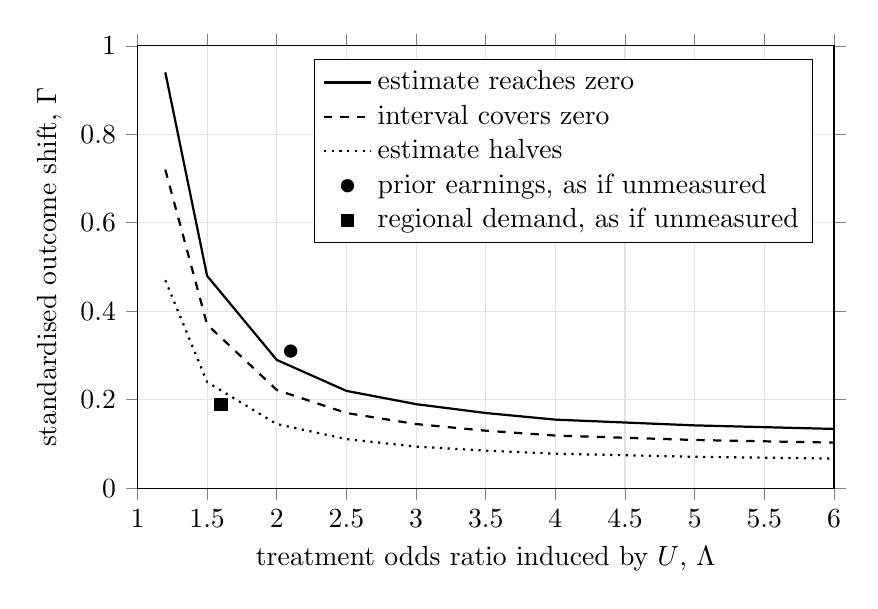
\begin{tikzpicture}
\begin{axis}[
  width=0.86\textwidth, height=7.2cm,
  xlabel={treatment odds ratio induced by $U$, $\Lambda$},
  ylabel={standardised outcome shift, $\Gamma$},
  xmin=1, xmax=6, ymin=0, ymax=1.0,
  legend pos=north east, legend cell align=left,
  grid=both, grid style={gray!22}, tick align=outside
]
\addplot[thick] coordinates {
  (1.2,0.94) (1.5,0.48) (2.0,0.29) (2.5,0.22) (3.0,0.19)
  (3.5,0.17) (4.0,0.155) (5.0,0.142) (6.0,0.134)
};
\addlegendentry{estimate reaches zero}
\addplot[thick,dashed] coordinates {
  (1.2,0.72) (1.5,0.37) (2.0,0.222) (2.5,0.170) (3.0,0.145)
  (3.5,0.130) (4.0,0.119) (5.0,0.109) (6.0,0.103)
};
\addlegendentry{interval covers zero}
\addplot[thick,dotted] coordinates {
  (1.2,0.47) (1.5,0.24) (2.0,0.145) (2.5,0.111) (3.0,0.094)
  (3.5,0.085) (4.0,0.078) (5.0,0.071) (6.0,0.067)
};
\addlegendentry{estimate halves}
\addplot[only marks,mark=*,mark size=2.2pt] coordinates {(2.1,0.31)};
\addlegendentry{prior earnings, as if unmeasured}
\addplot[only marks,mark=square*,mark size=2.2pt] coordinates {(1.6,0.19)};
\addlegendentry{regional demand, as if unmeasured}
\end{axis}
\end{tikzpicture}
\caption[Sensitivity contours for the retraining estimate]{Sensitivity contours
for the cross fitted AIPW estimate of Table~\ref{tab:dr-comparison}. A
confounder in the region above a curve is strong enough to produce the
corresponding change. The two plotted points are benchmarks: each is the
$(\Lambda, \Gamma)$ pair that a measured covariate would exhibit if it were
removed from the adjustment set.}
\label{fig:sensitivity-contours}
\end{figure}

Figure~\ref{fig:sensitivity-contours} is read by locating a plausible confounder
and checking which curves lie below it. The benchmark points make the exercise
concrete. Prior earnings, if it were unmeasured, would sit at
$(\Lambda, \Gamma) = (2.1, 0.31)$, comfortably above the solid curve, so a
single unmeasured confounder as strong as prior earnings would suffice to
eliminate the estimated effect. Regional demand, at $(1.6, 0.19)$, sits below
the solid curve and above the dotted one: it could halve the estimate but not
erase it.

\begin{remark}
\label{rem:benchmark-honesty}
Benchmarking\index{benchmarking} against measured covariates is the most defensible part of a
sensitivity analysis and the part most often omitted. The alternative, quoting a
value of $\Lambda$ chosen because it sounds large, invites the reader to accept
a number they have no way to calibrate.
\end{remark}

\section{Benchmark against an experiment}
\label{sec:sens-benchmark}

The retraining programme was randomised in two of its eleven regions in the
first year of operation, giving an experimental benchmark of 1290 units of
annual earnings with a standard error of 310. The observational estimate from
the remaining nine regions is 1418 with a standard error of 147.

\begin{table}[t]
\centering
\caption[Observational estimates against the experimental benchmark]{Adjusted
observational estimates from the nine non randomised regions compared with the
experimental benchmark from the two randomised regions. The bias column is
relative to the experimental point estimate. The final row applies the
sensitivity correction implied by the benchmark points of
Figure~\ref{fig:sensitivity-contours}.}
\label{tab:benchmark}
\begin{tabular}{lrrr}
\toprule
Specification & Estimate & Bias & Bias / std. error \\
\midrule
Experimental benchmark            & 1290 & --   & --   \\
Unadjusted difference             & 3184 & 1894 & 6.11 \\
Linear regression, main effects   & 1372 & 82   & 0.47 \\
Hajek weighting                   & 1461 & 171  & 0.44 \\
AIPW, cross fitted                & 1418 & 128  & 0.87 \\
AIPW plus completion covariate    & 2180 & 890  & 5.32 \\
AIPW with sensitivity correction  & 1301 & 11   & 0.06 \\
\bottomrule
\end{tabular}
\end{table}

Table~\ref{tab:benchmark} supports two conclusions and undermines a third. The
adjusted estimators all land within one standard error of the benchmark, which
is evidence that the measured covariates capture most of the confounding in this
setting. The specification that conditions on programme completion is badly
biased, exactly as Example~\ref{ex:collider} predicted, and its bias is of the
same order as the unadjusted contrast despite using more covariates.

The conclusion it undermines is that agreement with a benchmark validates a
method \citep{weiss2014benchmark}. Two randomised regions supply an estimate with a standard error of 310,
and a benchmark that wide cannot distinguish among estimators separated by 90
units. What the comparison rules out is gross failure, and that is all it rules
out.
